\documentclass[../projekt.tex]{subfiles}
\begin{document}
%=========================================================================
% (c) Michal Bidlo, Bohuslav Křena, 2008

\section{Úvod}\label{uvod}

Cílem tohoto projektu je návrh a implementace demonstrační aplikace Kargerova algoritmu pro nalezení minimálního řezu. Daný algoritmus byl navržen a implementován s využitím vhodných doporučených nástrojů. 




\section{Návrh aplikace}

Předběžný návrh aplikace je důležitým krokem ve vývoji. Při tomto postupu je možno se vyhnout případným problémům, které by mohly nastat v pozdější fázi vývoje. Prvním krokem byl návrh základního rozložení hlavního okna aplikace.  \\

	\begin{figure}[ht]
    	\begin{center}
  			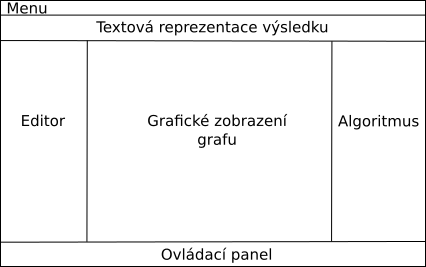
\includegraphics[scale=0.7]{obrazky-figures/layout.png}
  			\caption{Uspořádání hlavního okna aplikace.}
  			\label{fig:layout}
  		\end{center}
	\end{figure}

\subsection{Použité nástroje}

Dalším krokem návrhu aplikace byl výběr programovacího jazyka, ve kterém bude aplikace napsána. Výsledná aplikace by měla mít grafické rozhraní (GUI) a měla by být spustitelná na jakékoliv platformě, především na studentském serveru Merlin. Na základě těchto kritérii byl zvolen jazyk Java spolu s knihovnou Swing pro tvorbu grafického rozhraní. Ze seznamu povolených formátů grafů byl vybrán formát mxGraph a knihovna JGraphX s tímto formátem pracující. \\

\noindent\textbf{Swing} 

Swing \cite{swing} je knihovna plně založená na platformě Java a postavená na AWT (Abstract Windowing Toolkit), sloužící k ovládání počítače pomocí grafického rozhraní. S využitím této knihovny je možno vytvářet okna (JFrame), dialogy (JOptionPane), tlačítka (JButton), seznamy  a mnoho dalšího. \\


\noindent\textbf{JGraphX} 

JGraphX \cite{jgraphx} je knihovna licencovaná pod licencí BSD, založená na Java Swing knihovně, poskytující funkcionalitu pro vizualizaci a interakci s grafy založenými na systému uzel-hrana. JGraphX také obsahuje funkce pro podporu XML šablon, různých importů a exportů a rozvržení grafu.






\section{Implementace}

Hlavní částí vývoje byla implementace algoritmu podle zvolené varianty zadání, v případě tohoto projektu o Kargerův algoritmus. 

\subsection{Algoritmus}

Jedná se o deterministický randomizovaný algoritmus, který náhodně vybírá hranu mezi všemi hranami grafu a slučuje koncové uzly této hrany, dokud nezůstanou pouze dva super uzly \cite{karger}. Jednoduchý pseudokód hlavní smyčky programu: \\ 


\begin{algorithm}
\caption{Karger Algorithm}\label{euclid}
\begin{algorithmic}[1]
\State $Let \; G = (V, E)$
\While {$|V| > 2$}
\State $nahodne \; vyber \; dva \; sousedni \; uzly \; v1, \; v2$
\State $mergeCells(v1, \; v2)$
%\State $F \gets F\backslash E_{\overline{u}\overline{v}}$
\EndWhile
%\State $Return\, one\, of \,the\, supernodes\, in\, V \,and \,|E_{uv}|$
\end{algorithmic}
\end{algorithm}

\noindent a spojení dvou uzlů: \\

\begin{algorithm}
\caption{$mergeCells(v1,\; v2)$}\label{euclid}
\begin{algorithmic}[1]
%\State $x \gets new \, supernode$
%\State {$V(x) \gets V(a) \cup V(b) \; // merge \, the \, vertices$}
\ForEach { $v \in Adj[v2]$ }
\State $presmeruj \; uzel \; na \; v1$ 
%\State $V \ gets (V \backslash \{a,b\}) \ cup \{x\}$
\EndFor
\State $prejmenuj \; v1$ 
\State $odstran \; v2 \; a \; jeho \; hrany$ 

\end{algorithmic}
\end{algorithm}

Časová složitos Kargerova algoritmu je $O (n^4log \, n)$ vzhledem k tomu, že spuštíme $O (n^2log \, n)$ pokusů za $O(n^2)$ času \cite{karger}. 




\subsection{Struktura aplikace}

Celá aplikace je tvořena jedním hlavním oknem MainWindow. Rozložení hlavního okna je zobrazeno v návrhu aplikace na obrázku \ref{fig:layout}. Po spuštění aplikace proběhne načtění a zobrazení výchozího grafu. Uživatel má možnost vybrat pro zpracování jiný graf. Graf je možno editovat přidáním nebo odebráním uzlů a hran. Případná komunikace s uživatelem je realizována prostřednictvím dialogových oken. 


	\begin{figure}[ht]
    	\begin{center}
  			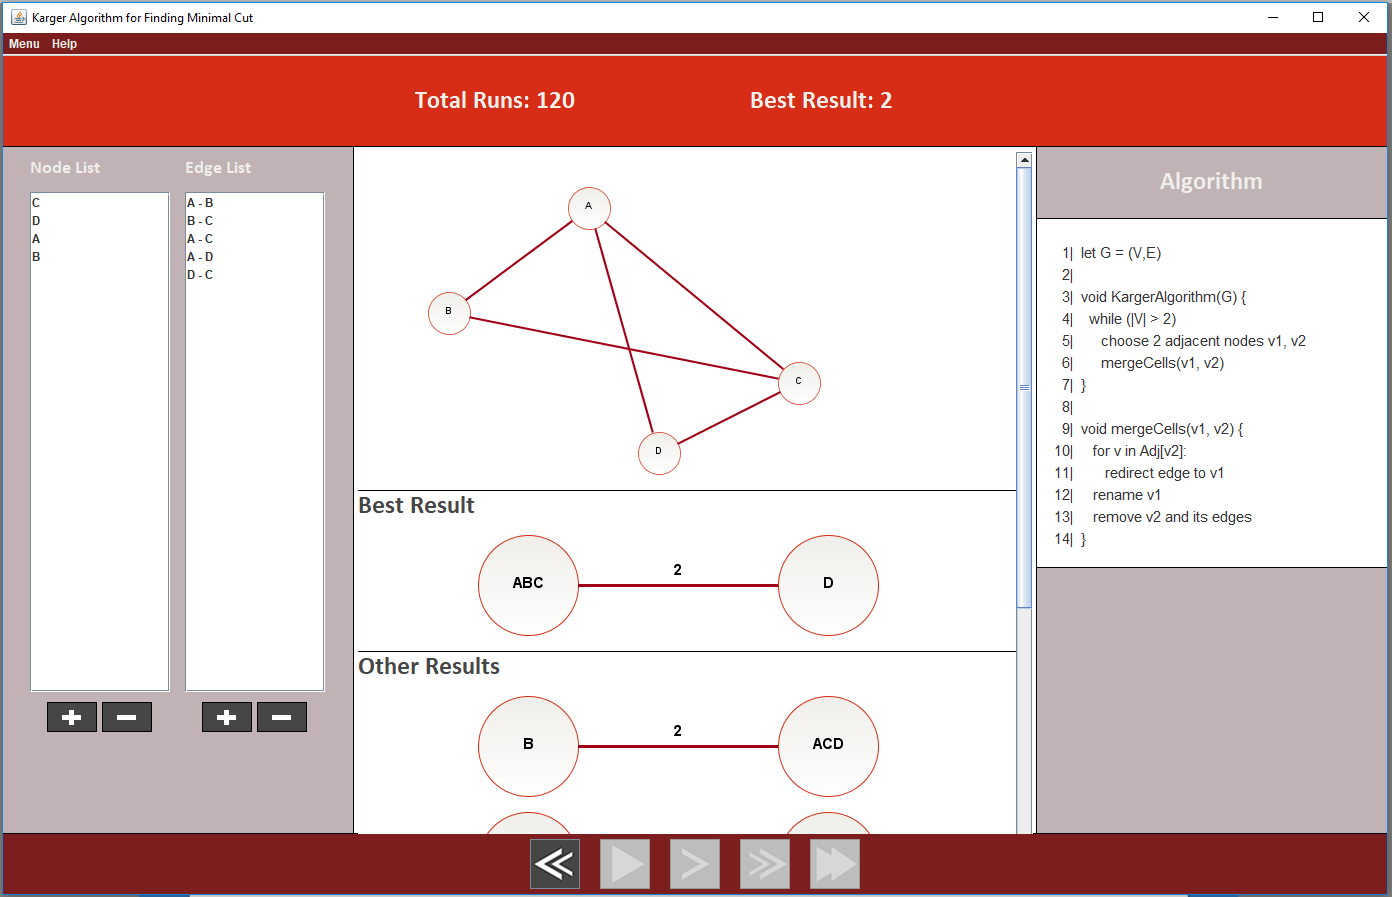
\includegraphics[scale=0.4]{obrazky-figures/finish.png}
  			\caption{Zobrazení výsledku aplikace algoritmu na daný graf.}
  		\end{center}
	\end{figure}



\newpage
\section{Aplikace}

% seznam minimalnich pozadavku
\subsection{Minimální požadavky}

\begin{itemize}
	\item OpenJDK
	\item Ant 
	\item JGraphX
\end{itemize}


\subsection{Spuštění a instalace}

Odevzdaný archiv obsahuje:

\begin{itemize}
	\item src - adresář se zdrojovými soubory
	\item lib - adresář s využitými knihovnami
	\item latex - zdrovojé kódy této dokumentace 
	\item README.md
	\item dokumentace.pdf - tato dokumentace 
	\item build.xml - skript pro kompilaci a spuštění aplikace pomocí Ant
\end{itemize}

\noindent Pro sputění aplikace je nutno mít nainstalovaný OpenJDK a Java knihovnu Apache Ant. Aplikace se spouští přes soubor karger.jar.


% kratky uvodni popis moznosti aplikace
\subsection{Možnosti aplikace}

\begin{itemize}
	\item Vytvoření/načtení/uložení grafu ve formátu XML,
	\item editace grafu - přidání a odebrání uzlu/hrany,
	\item ovládání grafu pomocí ovládacího panelu - reset, další krok, dokončení jednoho běhu, dokončení, algoritmu
	\item podrobnější krokování provádění algoritmu spoulu s vyznačením právě provedených částí pseudokódu,
	\item přesun uzlů pomocí kliknutí a tažení myší,
	\item zobrazení uživatelského manuálu pod záložkou help v horním menu.
\end{itemize}



\section{Závěr}

Cílem práce bylo vytvořit aplikaci, která demonstruje Kargerův algoritmus pro nalezení minimálního řezu. Samotné řešení projektu s využitím knihovny JGraphX bylo poučné a vedlo k pochopení fungování Kargerova algoritmu. Výsledná aplikace je vydařená a toto řešení by mělo uživateli pomoci minimálně s pochopením základního principu algoritmu.

\end{document}